\documentclass[
  bibliography=totoc,     % Literatur im Inhaltsverzeichnis
  captions=tableheading,  % Tabellenüberschriften
  titlepage=firstiscover, % Titelseite ist Deckblatt
]{scrartcl}

% Paket float verbessern
\usepackage{scrhack}

% Warnung, falls nochmal kompiliert werden muss
\usepackage[aux]{rerunfilecheck}

% unverzichtbare Mathe-Befehle
\usepackage{amsmath}
% viele Mathe-Symbole
\usepackage{amssymb}
% Erweiterungen für amsmath
\usepackage{mathtools}

% Fonteinstellungen
\usepackage{fontspec}
% Latin Modern Fonts werden automatisch geladen
% Alternativ zum Beispiel:
%\setromanfont{Libertinus Serif}
%\setsansfont{Libertinus Sans}
%\setmonofont{Libertinus Mono}

% Wenn man andere Schriftarten gesetzt hat,
% sollte man das Seiten-Layout neu berechnen lassen
\recalctypearea{}

% deutsche Spracheinstellungen
\usepackage[ngerman]{babel}


\usepackage[
  math-style=ISO,    % ┐
  bold-style=ISO,    % │
  sans-style=italic, % │ ISO-Standard folgen
  nabla=upright,     % │
  partial=upright,   % ┘
  warnings-off={           % ┐
    mathtools-colon,       % │ unnötige Warnungen ausschalten
    mathtools-overbracket, % │
  },                       % ┘
]{unicode-math}

% traditionelle Fonts für Mathematik
\setmathfont{Latin Modern Math}
% Alternativ zum Beispiel:
%\setmathfont{Libertinus Math}

\setmathfont{XITS Math}[range={scr, bfscr}]
\setmathfont{XITS Math}[range={cal, bfcal}, StylisticSet=1]

% Zahlen und Einheiten
\usepackage[
  locale=DE,                   % deutsche Einstellungen
  separate-uncertainty=true,   % immer Fehler mit \pm
  per-mode=symbol-or-fraction, % / in inline math, fraction in display math
]{siunitx}

% chemische Formeln
\usepackage[
  version=4,
  math-greek=default, % ┐ mit unicode-math zusammenarbeiten
  text-greek=default, % ┘
]{mhchem}

% richtige Anführungszeichen
\usepackage[autostyle]{csquotes}

% schöne Brüche im Text
\usepackage{xfrac}

% Standardplatzierung für Floats einstellen
\usepackage{float}
\floatplacement{figure}{htbp}
\floatplacement{table}{htbp}

% Floats innerhalb einer Section halten
\usepackage[
  section, % Floats innerhalb der Section halten
  below,   % unterhalb der Section aber auf der selben Seite ist ok
]{placeins}

% Seite drehen für breite Tabellen: landscape Umgebung
\usepackage{pdflscape}

% Captions schöner machen.
\usepackage[
  labelfont=bf,        % Tabelle x: Abbildung y: ist jetzt fett
  font=small,          % Schrift etwas kleiner als Dokument
  width=0.9\textwidth, % maximale Breite einer Caption schmaler
]{caption}
% subfigure, subtable, subref
\usepackage{subcaption}

% Grafiken können eingebunden werden
\usepackage{graphicx}
% Für Dateinamen mit mehreren Punkten (z.B. .eps.gz)
% \usepackage{grffile} % Currently broken, See ho-tex/oberdiek#73

% schöne Tabellen
\usepackage{booktabs}

% Verbesserungen am Schriftbild
\usepackage{microtype}

% Literaturverzeichnis
\usepackage[
  backend=biber,
]{biblatex}
% Quellendatenbank
\addbibresource{lit.bib}
\addbibresource{programme.bib}

% Hyperlinks im Dokument
\usepackage[
  german,
  unicode,        % Unicode in PDF-Attributen erlauben
  pdfusetitle,    % Titel, Autoren und Datum als PDF-Attribute
  pdfcreator={},  % ┐ PDF-Attribute säubern
  pdfproducer={}, % ┘
]{hyperref}
% erweiterte Bookmarks im PDF
\usepackage{bookmark}

% Trennung von Wörtern mit Strichen
\usepackage[shortcuts]{extdash}

\author{%
  Nikola Sarah Mang\\%
  \and%
  Mirjam Prayer\\%
}
\publishers{TU Dortmund – Fakultät Physik}


\subject{V354}
\title{Gedämpfte und erzwungene Schwingungen}
\date{%
  Durchführung: 27.04.2021
  \hspace{3em}
  Abgabe: 03.05.2021
}

\begin{document}

\maketitle
\thispagestyle{empty}
\tableofcontents
\newpage

\section{Theorie}
\label{sec:Theorie}

\subsection{Relaxationsverhalten des RC-Kreises}
    Zwischen den Platten eines Kondesators liegt die Spannung 
    \begin{equation}
        \label{eq:sp}
        U_C = \dfrac{Q}{C}
    \end{equation} an.
    Beim Ausgleich der Ladungen, sprich der Entladung des Kondensators entseht der 
    Strom 
    \begin{equation}
        \label{eq:st}
        I = \dfrac{U_C}{R}.
    \end{equation}
    Aus dem Zusammenhang $dQ=-I\ dt$ kann durch Einsetzen von \ref{eq:sp} und \ref{eq:st}
    die Differentialgleichung 
    \begin{equation}
        \dfrac{dQ}{dt}= -\dfrac{1}{RC} Q{t}
    \end{equation}
    gewonnen werden. Der Entladevorgang lässt sich offensichtlich durch 
    \begin{equation}
        \label{eq:dgl}
        Q(t)=Q(0)e^{\dfrac{-t}{RC}}
    \end{equation}
    beschreiben. Der die DGL ebenfalls lösende Term mit positivem Exponenten entfällt aufgrund der 
    Bedingung $Q(\infty)=0$.\\
    Für den Aufladevorgang gilt die gleiche Differentialgleichung \ref{eq:dgl}. Ledeglich die
    Randbedingungen lauten nun $Q(0)=0$ und $Q(\infty)=CU_0$. Unter diesen Bedingungen lässt sich 
    die Differentialgleichung durch 
    \begin{equation}
        Q(t) = CU_0(1-e^{\dfrac{-t}{RC}})
    \end{equation}
    lösen.\\
    Die Zeitkonstante RC ist ein Maß für die Relaxationsgeschwindigkeit. Während des 
    Zeitintervalls $\Delta T=RC$ sinkt die Ladung des Kondensators um den Faktor
    $\dfrac{Q(t=RC)}{Q(0)}=\dfrac{1}{e}$.

\subsection{Relaxationsverhalten unter Einfluss angelegter periodischer Spannung}
    Ist die Frequenz der angelegten Wechselspannung $U(t)=U_0\cos{\omega t}$ sehr niedrig,
    so verhält sich $U_C(t)$ wie $U(t)$. Bei höheren Frequenzen verzögert sich 
    die Auf- und Entladung des Kondensators durch den Widerstand, sodass eine 
    Phasenverschiebung $\phi$ zwischen dem Kondensator und der Spannungsquelle 
    entsteht. Dadurch verringert sich auch die Amplitude der Kondensatorspannung.
    im folgenden wird für die Kondensatorspannung der Ansatz $U_C(t)=A(\omega)
    \cos{\omega t + \phi{\omega}}$ verwendet.
    \begin{figure}[H]
        \centering
        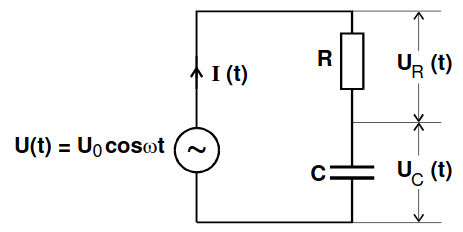
\includegraphics{schalt3.png}
        \caption{Der RC-Schaltkreis mit angelegter Cosinus-Spannung}
        \label{fig:schalt3}
    \end{figure}
    Die Spannung des in Abbildung \ref{fig:schalt3} dargestellten Stromkreises kann nach dem zweiten
    Kirchhoffschen Gesetzt durch 
    \begin{equation}
        \label{eq:kirsche}
        U(t)=U_R(t)+U_C(t) \Leftrightarrow U_0 \cos{\omega t}=I(t)R + 
        A(\omega)\cos{\omega t + \phi}
    \end{equation}
    bestimmt werden. Wird sich nun ernaut des Zusammenhangs $\dfrac{dQ}{dt}=-I$ und 
    Gleichung \ref{eq:sp} bedient, ergibt sich
    \begin{equation}
        U_0\cos{\omega t}=-A(\omega)\omega RC \sin{\omega t+\phi}+A(\omega)\cos{\omega t + \phi}
    \end{equation}
    Wird nun $\omega=\dfrac{\pi}{2}$ gesetzt, wird diese Gleichung zu 
    \begin{equation*}
        0 = -\omega RC \sin{\dfrac{\pi}{2} + \phi}+\cos{\dfrac{\pi}{2}+\phi}
    \end{equation*}
    Wird nun ausgenützt, dass $\sin{\phi + \dfrac{\pi}{2}}$, entsteht die Betiehung
    \begin{equation}
        \label{eq:phi}
        \phi(\omega)=\arctan{-\omega RC}
    \end{equation}
    zwischen Phase und verwendeter Frequenz. Nun wird der der Fall $\omega t + \phi = 
    \dfrac{\pi}{2}$ betrachtet. Es gilt
    \begin{align*}
        U_0 \cos{\dfrac{\pi}{2}-\phi}=-A(\omega)\omega RC\\
        \Leftrightarrow A(\omega)=-\dfrac{\sin{\phi}}{\omega RC}U_0
    \end{align*}
    Unter Verwendung von \ref{eq:phi} kann die Beziehung $\sin{\phi}=\dfrac{\omega RC}
    {\sqrt{1+\omega^2 R^2 C^2}}$ hergeleitet und in die Gleichung eingesetzt werden.
    Dadurch ergibt sich 
    \begin{equation}
        A(\omega)=\dfrac{U_0}{\sqrt{1+\omega^2 R^2 C^2}}
    \end{equation}
    Während kleine Frequanzen nur eine geringe Abweichung von der angelegten Spannung
    aufweisen, verschwindet die Amplitude für sehr große Frequenzen.
    RC-Glieder stellen also einen Tiefpass im elektrischen Schaltkreis dar.

\subsection{Der RC-Kreis als Integrator}
    Ein anderer möglicher Effekt des RC-Kreises ist die Integration der Spannung. Wir betrachten 
    erneut Gleichung \ref{eq:kirsche}.
    \begin{equation*}
        U(t)=U_R(t)+U_C(t)=I(t)R+U_C(t)=RC\dfrac{dU_C}{dt}+U_C(t)
    \end{equation*} 
    Falls nun $\omega \ll \dfrac{1}{RC}$ ist die Spannung $\vert U_C \vert \ll \vert U_R \vert$
    Näherungsweise ist dann 
    \begin{equation}
        \U(t)=RC\dfrac{dU_C}{dt} \Leftrightarrow U_C(t)=\dfrac{1}{RC}\int_0^t U(t')dt'.
    \end{equation}

\section{Durchführung}
\label{sec:Durchführung}

Die verwendete Apperatur ist in Abbildung ... schematisch dargestellt. Sie besteht aus 
einer Spannvorrichtung in Punkt A sowie zwei Auflagepunkten A und B, die %dong 
cm voneinander entfernt sind.
Nun gibt es zwei vertikal fest intergrierte Messvorichtungen, die in horizontaler Richtung 
verschiebbar sind.
\begin{figure}
    \centering
    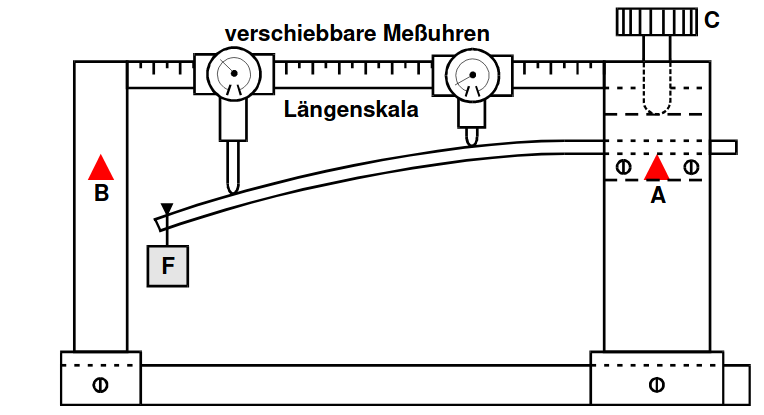
\includegraphics[scale=0.5]{panierte Austern.png}
    \caption{Schematische Darstellung einer Apparatur zur Vermessung elastisch gebogener Stäbe}
    \label{fig:backfisch}
\end{figure}

\subsection{Einseitiges Einspannen}
    Mittels der Spannvorrichtung an Punkt A werden zwei Stäbe verschiedenen Materials
    eingespannt. Um Fehlerquellen wie Vorbiegung des Stabes oder eine nicht parallele
    Ausrichtung der Messgeräte vorzubeugen, wird jeweils die Differenz der Auslenkung
    bei Normalzustand und im Zustand mit angehängtem Gewicht gemessen.\\
    Bei der ersten Messreihe mit einem viereckigen Stab wird in einer Entfernung von %dong
    cm ein Gewicht von %dong kg befestigt.
    Bei der ersten Messreihe mit einem viereckigen Stab wird in einer Entfernung von %dong
    cm ein Gewicht von %dong kg befestigt.
    Die Messwerte wurden in der Nähe der Einspannung im 5 cm Abstand und in der Nähe
    des Gewichtes im 2 cm Abstand genommen.


\subsection{Beidseitige Auflage}
    Die zu untersuchende Probe wird auf den Fußpunkten A und B gelagert. 
    

    Die Messwerte wurden in der Nähe der Einspannung im 5 cm Abstand und in der Nähe
    des Gewichtes im 2 cm Abstand genommen.
\section{Auswertung}
\label{sec:Auswertung}

\subsection{Vanadium}
Als Erstes sollte die Untergrundrate ermittelt werden, dazu wurde in 
$300 \si{\s}$-Intervallen die Zerfallsrate gemessen. So ergaben sich
$N_U = {129, 143, 144, 136, 126, 158}$.

Anschließend wurde der Zerfall von $^{52}V$ gemessen. Dabei handelt sich um 
ein Isotop mit einfachem Zerfall. Als Zeitintervall wurde $\increment t = 30 \si{\s}$
geewählt, sodass sich die in Tabelle \ref{tab:vanwerte} ergaben. Die Fehler wurden dabei 
durch die Poisson-Verteilung $\increment N = \sqrt{N}$ ermittelt.

\begin{table}
 \centering
 \caption{Messdaten für den Zerfall von Vanadium.}
 \label{tab:vanwerte}
 \begin{tabular}{c c c}
  \toprule
  {$t \mathbin{/} \si{\s}$} & {$N_{\increment t, \text{gem}}$} & {$\increment N_{\increment t, \text{gem}}$}\\
  \midrule
  30.0                 & 189.0                & 13.74  \\
  60.0                 & 197.0                & 14.03  \\
  90.0                 & 150.0                & 12.24  \\
  120.0                & 159.0                & 12.60  \\
  150.0                & 155.0                & 12.44  \\
  180.0                & 132.0                & 11.48  \\
  210.0                & 117.0                & 10.81  \\
  240.0                & 107.0                & 10.34  \\
  270.0                & 94.0                 & 9.695  \\
  300.0                & 100.0                & 10.0   \\
  330.0                & 79.0                 & 8.888  \\
  360.0                & 69.0                 & 8.306  \\
  390.0                & 81.0                 & 9.0    \\
  420.0                & 46.0                 & 6.782  \\
  450.0                & 49.0                 & 7.0    \\
  480.0                & 61.0                 & 7.810  \\
  510.0                & 56.0                 & 7.483  \\
  540.0                & 40.0                 & 6.324  \\
  570.0                & 45.0                 & 6.708  \\
  600.0                & 32.0                 & 5.656  \\
  630.0                & 27.0                 & 5.196  \\
  660.0                & 43.0                 & 6.557  \\
  690.0                & 35.0                 & 5.916  \\
  720.0                & 19.0                 & 4.358  \\
  750.0                & 28.0                 & 5.291  \\
  780.0                & 27.0                 & 5.196  \\
  810.0                & 36.0                 & 6.0    \\
  840.0                & 25.0                 & 5.0    \\
  870.0                & 29.0                 & 5.385  \\
  900.0                & 18.0                 & 4.242  \\
  930.0                & 17.0                 & 4.123  \\
  960.0                & 24.0                 & 4.898  \\
  990.0                & 21.0                 & 4.582  \\
  1020.0               & 25.0                 & 5.0    \\
  1050.0               & 21.0                 & 4.582  \\
  1080.0               & 24.0                 & 4.898  \\
  1110.0               & 25.0                 & 5.0    \\
  1140.0               & 17.0                 & 4.123  \\
  1170.0               & 20.0                 & 4.472  \\
  1200.0               & 19.0                 & 4.358  \\
  1230.0               & 20.0                 & 4.472  \\
  1260.0               & 18.0                 & 4.242  \\
  1290.0               & 16.0                 & 4.0    \\
  1320.0               & 17.0                 & 4.123  \\
  \bottomrule
 \end{tabular}
\end{table}

\noindent Mithilfe des Mittelwertes der Messung für den Untergrund $N_U = \pm $
folgen die wahren Werte für $N_{\increment t}$ wie in Tabelle \ref{tab:vanwahr} 
aufgeführt.

\begin{table}
 \centering
 \caption{Messwerte von Vanadium ohne Untergrundrate.}
 \label{tab:vanwahr}
 \begin{tabular}{c c c}
  \toprule
  {$t \mathbin{/} \si{\s}$} & {$N_{\increment t}$} & {$\increment N_{\increment t}$}\\
  \midrule
  30.0    & 175.066  & 13.831  \\
  60.0    & 183.066 & 14.118  \\
  90.0    & 136.066  & 12.341  \\
  120.0   & 145.066  & 12.701  \\
  150.0   & 141.066  & 12.542  \\
  180.0   & 118.066  & 11.589  \\
  210.0   & 103.066  & 10.923  \\
  240.0   & 93.066  & 10.455  \\
  270.0   & 80.066  & 9.814  \\
  300.0   & 86.066  & 10.115  \\
  330.0   & 65.066  & 9.017\\
  360.0   & 55.066  & 8.445  \\
  390.0   & 67.066  & 9.128  \\
  420.0   & 32.066  & 6.951  \\
  450.0   & 35.066  & 7.163  \\
  480.0   & 47.066  & 7.957  \\
  510.0   & 42.066  & 7.636  \\
  540.0   & 26.066  & 6.505  \\
  570.0   & 31.066  & 6.879  \\
  600.0   & 18.066  & 5.858  \\
  630.0   & 13.066  & 5.414  \\
  660.0   & 29.066  & 6.732  \\
  690.0   & 21.066  & 6.109  \\
  720.0   & 5.066  & 4.617  \\
  750.0   & 14.066  & 5.506  \\
  780.0   & 13.066  & 5.414  \\
  810.0   & 22.066  & 6.190  \\
  840.0   & 11.066  & 5.227  \\
  870.0   & 15.066  & 5.596  \\
  900.0   & 4.066  & 4.508  \\
  930.0   & 3.066  & 4.395  \\
  960.0   & 10.06  & 5.130  \\
  990.0   & 7.066  & 4.829  \\
  1020.0  & 11.06  & 5.227  \\
  1050.0  & 7.066  & 4.829  \\
  1080.0  & 10.06  & 5.130  \\
  1110.0  & 11.06  & 5.227  \\
  1140.0  & 3.066  & 4.395  \\
  1170.0  & 6.066  & 4.724  \\
  1200.0  & 5.066  & 4.617  \\
  1230.0  & 6.066  & 4.724  \\
  1260.0  & 4.066  & 4.508  \\
  1290.0  & 2.066  & 4.280  \\
  1320.0  & 3.066  & 4.395  \\
  \bottomrule
 \end{tabular}
\end{table}

\noindent Aus diesen Werten wurde mithilfe einer linearen Regression
eine Kurve für den Zerfall von Vanadium errechnet, nach Formel %\eqref{eqn:}
aus der Theorie. Es gilt:
\begin{align*}
    \lambda = (0.323 \pm 0.011) \cdot 10^(-2) \\
    c = 5.32 \pm 0.04 \\
    ln(N_{\increment t}) = c - \lambda t 
\end{align*}
Aus dem Zerfallsparameter $\lambda$ lässt sich die Halbwertszeit $T_V$ von
Vanadium berechnen nach %\ref{}.
\begin{equation*}
    T_V = 215+/-7 \si{\s}
\end{equation*}
Eine genauere Methode nimmt nicht alle Werte in die lineare Regression auf,
dazu wurden alle Wertepaare nach der doppelten Halbwertszeit vernachlässigt.
Es folgt
\begin{align*}
    \lambda_2 = (0.333 \pm 0.022) \cdot 10^(-2) \\
    c_2 = 5.34 \pm 0.05 \\
    ln(N_{\increment t}) = c_2 - \lambda_2 t \\
    T_V,2 = 208+/-13
\end{align*}
Abbildung \ref{fig:vankurve}
zeigt die Messwerte ohne Untergrund sowie die beiden linearen Regressionen.

\begin{figure}
 \centering
 \includegraphics[width=\textwidth]{Vanadium.pdf}
 \caption{Messdaten und Fits für den Zerfall von Vanadium.}
 \label{fig:vankurve}
\end{figure}

\subsection{Rhodium}

Für die Messung des Zerfalls von Rhodium wurde ein Zeitintervall von 
$\increment t = 15 \si{\s}$ gewählt. Die Messdaten sind in Tabelle \ref{tab:rhowerte}
aufgelistet.

\begin{table}
 \centering
 \caption{Messwerte von Rhodium.}
 \label{tab:rhowerte}
 \begin{tabular}{c c c}
  \toprule
  {$t \mathbin{/} \si{\s}$} & {$N_{\increment t, \text{gem}}$} & {$\increment N_{\increment t, \text{gem}}$}\\
  \midrule
  15.0    & 667.0  & 25.826 \\
  30.0    & 585.0  & 24.186  \\  
  45.0    & 474.0  & 21.771  \\  
  60.0    & 399.0  & 19.974  \\  
  75.0    & 304.0  & 17.435  \\  
  90.0    & 253.0  & 15.905  \\  
  105.0   & 213.0  & 14.594  \\  
  120.0   & 173.0  & 13.152  \\  
  135.0   & 152.0  & 12.328  \\  
  150.0   & 126.0  & 11.224  \\  
  165.0   & 111.0  & 10.535  \\  
  180.0   & 92.0   & 9.591  \\  
  195.0   & 79.0   & 8.888  \\  
  210.0   & 74.0   & 8.602  \\  
  225.0   & 60.0   & 7.745  \\  
  240.0   & 52.0   & 7.211  \\  
  255.0   & 56.0   & 7.483  \\  
  270.0   & 53.0   & 7.280  \\  
  285.0   & 41.0   & 6.403  \\  
  300.0   & 36.0   & 6.0     \\  
  315.0   & 37.0   & 6.082  \\  
  330.0   & 32.0   & 5.656  \\  
  345.0   & 36.0   & 6.0    \\  
  360.0   & 38.0   & 6.164  \\  
  375.0   & 34.0   & 5.830  \\  
  390.0   & 40.0   & 6.324  \\  
  405.0   & 21.0   & 4.582  \\  
  420.0   & 35.0   & 5.916  \\  
  435.0   & 33.0   & 5.744  \\  
  450.0   & 36.0   & 6.0     \\  
  465.0   & 20.0   & 4.472  \\  
  480.0   & 24.0   & 4.898  \\  
  495.0   & 30.0   & 5.477  \\  
  510.0   & 30.0   & 5.477  \\  
  525.0   & 26.0   & 5.099  \\  
  540.0   & 28.0   & 5.291  \\  
  555.0   & 23.0   & 4.795  \\  
  570.0   & 20.0   & 4.472  \\  
  585.0   & 28.0   & 5.291  \\  
  600.0   & 17.0   & 4.123  \\  
  615.0   & 26.0   & 5.099  \\  
  630.0   & 19.0   & 4.358  \\  
  645.0   & 13.0   & 3.605  \\  
  660.0   & 17.0   & 4.123 \\
  \bottomrule
 \end{tabular}
\end{table} 

Nach abziehen der auf ein Zeitintervall von 15 Sekunden normierten Untergrundrate
bleiben die in Tabelle \ref{tab:rhowahr} 
gezeigten Daten.

\begin{table}
 \centering
 \caption{Messwerte von Rhodium ohne Untergrund.}
 \label{tab:rhowahr}
 \begin{tabular}{c c c}
  \toprule
  {$t \mathbin{/} \si{\s}$} & {$N_{\increment t}$} & {$\increment N_{\increment t}$}\\
  \midrule
  15.0   & 660.033  & 25.848    \\
  30.0   & 578.033  & 24.210  \\
  45.0   & 467.033  & 21.798  \\
  60.0   & 392.033  & 20.004  \\
  75.0   & 297.033  & 17.468  \\
  90.0   & 246.033  & 15.942  \\
  105.0  & 206.033  & 14.634  \\
  120.0  & 166.033  & 13.197  \\
  135.0  & 145.033  & 12.375  \\
  150.0  & 119.033  & 11.276  \\
  165.0  & 104.033  & 10.590  \\
  180.0  & 85.033  & 9.652  \\
  195.0  & 72.033  & 8.953  \\
  210.0  & 67.033  & 8.669  \\
  225.0  & 53.033  & 7.820  \\
  240.0  & 45.033  & 7.291  \\
  255.0  & 49.033  & 7.560  \\
  270.0  & 46.033  & 7.359  \\
  285.0  & 34.033  & 6.493  \\
  300.0  & 29.033  & 6.095  \\
  315.0  & 30.033  & 6.177  \\
  330.0  & 25.033  & 5.758  \\
  345.0  & 29.033  & 6.095  \\
  360.0  & 31.033  & 6.257  \\
  375.0  & 27.033  & 5.929  \\
  390.0  & 33.033  & 6.415  \\
  405.0  & 14.033  & 4.707  \\
  420.0  & 28.033  & 6.013  \\
  435.0  & 26.033  & 5.844  \\
  450.0  & 29.033  & 6.095  \\
  465.0  & 13.033  & 4.600  \\
  480.0  & 17.033  & 5.016  \\
  495.0  & 23.033  & 5.582  \\
  510.0  & 23.033  & 5.582  \\
  525.0  & 19.033  & 5.211  \\
  540.0  & 21.033  & 5.400  \\
  555.0  & 16.033  & 4.915  \\
  570.0  & 13.033  & 4.600  \\
  585.0  & 21.033  & 5.400  \\
  600.0  & 10.033  & 4.261  \\
  615.0  & 19.033  & 5.211  \\
  630.0  & 12.033  & 4.490  \\
  645.0  & 6.033   & 3.763  \\
  660.0  & 10.033  & 4.261 \\
  \bottomrule
 \end{tabular}
\end{table}

\noindent Nach Auftragen der Messwerte halblogarithmisch gegen die Zeit wie in Abbildung \ref{fig:messf},
ist eine Struktur erkennbar. Ab der Zeit $t_l = 270 \si{\s}$ ist nur noch der langsamere Zerfall
von Bedeutung, während der schnellere bis zur Zeit $t_s = 150 \si{\s}$ vorherrschend ist.

\begin{figure}
 \centering
 \includegraphics[width=\textwidth]{werte.pdf}
 \caption{Messwerte des Rhodiumzerfalls mit Fehlern.}
 \label{fig:messf}
\end{figure}

\noindent Für $t > t_l$ lässt sich die Kurve des langlebigen Zerfalls extrapolieren, sodass 
sie dargestellt werden kann mit
\begin{align*}
    \lambda_l = (0.323 \pm 0.11) \cdot 10^{-2}\\
    c_l = 4.35 \pm 0.17 \\
    ln(N_{langlebig}) = c_l - \lambda_l \cdot t
\end{align*}

Nach Abziehen des so erhaltenen Beitrages vom langlebigen Zerfall ist es möglich, auch
eine Darstellung des kurzlebigen Zerfalls zu finden. Sie wird wie folgt charakterisiert.
\begin{align*}
    \lambda_k = (1.61 \pm 0.04) \cdot 10^{-2}\\
    c_k = 6.678 \pm 0.025 \\
    ln(N_{langlebig}) = c_k - \lambda_k \cdot t
\end{align*}

Abbildung \ref{fig:regress} zeigt die jeweiligen Kurven für ihren Geltungsbereich sowie die Kombination aus beiden.

\begin{figure}
 \centering
 \includegraphics[width=\textwidth]{rhodium.pdf}
 \caption{Regressionskurven für den Zerfall von Rhodium.}
 \label{fig:regress}
\end{figure}

\noindent Als Halbwertszeiten ergeben sich aus den Zerfallskonstanten
\begin{align*}
    T_l = 258.149 \pm 0.001 \si{\s} \\
    T_k = 43.054 \pm 0.025 \si{\s}\\
\end{align*}
\section{Diskussion}
\label{sec:Diskussion}
Die Messwerte, die im Laufe des Versuches aufgenommen und ausgerechnet wurden,
lauten
\begin{align*}
R = 2.65 \si{\ohm} \\
\rho = 1.56 \cdot 10^{-8} \si{\ohm\m} \\
n_\text{Sk} = \left( 1.271 \pm 0.022 \right) \cdot 10^{29} \si{\per\m\cubed}\\
n_\text{Pk} = \left( 0.899 \pm 0.19 \right) \cdot 10^{29} \si{\per\m\cubed}\\
z_\text{Sk} = 1.501 \pm 0.026 \\
z_\text{Pk} = 1.061 \pm 0.023 \\
v_\text{d, Sk} = (4.91 \pm 0.09) \cdot 10^{-5} \si{\m\per\s}\\
v_\text{d, Pk} = (6.95 \pm 0.15)  \cdot 10^{-5} \si{\m\per\s}\\
\bar{\tau}_{Sk} = \left( 3.59 \pm 0.06 \right) \cdot 10^{-14} \si{\s}\\
\bar{\tau}_{Pk} = \left( 5.08 \pm 0.11 \right) \cdot 10^{-14} \si{\s}\\
\mu_{Sk} = \left( 3.16 \pm 0.06 \right) \cdot 10^{-2} \si{\m\squared\per\volt\s} \\
\mu_{Pk} = \left( 4.47 \pm 0.09 \right) \cdot 10^{-2}\si{\m\squared\per\volt\s} \\
\bar{v}_{Sk} = \left( 1.801 \pm 0.011 \right) \cdot 10^{6} \si{\m\per\s}\\
\bar{v}_{Pk} = \left( 1.604 \pm 0.011 \right) \cdot 10^{6} \si{\m\per\s}\\
\bar{l}_{Sk} = \left( 6.47 \pm 0.08 \right) \cdot 10^{-8} \si{\m}\\
\bar{l}_{Pk} = \left( 8.15 \pm 0.12 \right) \cdot 10^{-8} \si{\m}
\end{align*}

Tabelle \ref{tab:theo} zeigt die Theoriewerte und die prozentualen Abweichungen 
der jeweiligen Messreihen. Dabei stammen die Werte für die Ladungsträgersichte und
die Beweglichkeit aus Quelle \cite{beweglichkeit}, die für die Totalgeschwindigkeit,
die mittlere Flugzeit und die mittlere freie Weglänge aus \cite{transport}. 
\begin{table}[H]
 \centering
 \caption{Theoriewerte und prozentuale Abweichungen.}
 \label{tab:theo}
 \begin{tabular}{lccc}
  \toprule
   & & \multicolumn{2}{c}{Abweichungen in Prozent}\\
  \cmidrule(lr){3-4}
  Messwert & Theoriewert & Spulenstrom konst. & Probenstrom konst. \\
  \midrule
  Ladungsträgersichte n & $1 \cdot 10^{29} \si{\per\m\cubed}$ & 2.7 & 1.0\\
  $\bar{\tau}$ & $2.51 \cdot 10^{-14} \si{s}$ & 4.3 & 10.2\\
  Beweglichkeit $\mu$ & $4.36 \cdot 10^{-3} \si{\m\squared\per\volt\s}$ & 2.7 & 0.2 \\
  Totalgeschwindigkeit $\bar{v}$ & $1.6 \cdot 10^{6} \si{\m\per\s}$ & 1.2 & 0.3 \\
  mittlere freie Weglänge & $4.02 \cdot 10^{-8} \si{\m}$ & 6.1 & 10.2 \\
  \bottomrule
 \end{tabular}
\end{table}
\noindent Der Theoriewert für den spezifischen Widerstand beträgt nach \cite{spezid} 
$\rho_\text{Theorie} = 1.75 \cdot 10^{-8} \si{\ohm\m}$, also folgt eine prozentuale 
Abweichung von 10 Prozent.\\
Die Abweichungen sind im Allgemeinen gering, dennoch lässt sich eine Diskrepanz feststellen.
Eine mögliche Ursache für Messunsicherheiten ist, dass die Messung des Stroms sehr ungenau
war, da die Ströme sehr klein waren und schon im Millivolt-Bereich nur 
die dritte Nachkommastelle gemessen wurde. Diese Ungenauigekeit zieht sich
natürlich durch die komplette Rechnung durch.\\
Zudem hat es der Generator nicht immer geschafft, auf $5 \si{\A}$ hochzuregeln
und so sind die Werte, mit denen für 5 Ampere gerechnet wurde, nicht immer einwandfrei
vergleichbar. \\
Da digitale Messgeräte zur Messung der Spannung und des Magnetfeldes verwendet
wurden, ist zu erwarten, dass der menschliche Fehler bei diesen Werten eine geringere
Rolle spielt.\\
Da bei der Herleitung der Formeln einige Näherungen gemacht wurden, sind ebenfalls
Abweichungen zu Erwarten.
Zwischen den jeweiligen Messreihen ist kein deutlicher Unterschied festzustellen.

\printbibliography{}
\begin{figure}
  \centering
  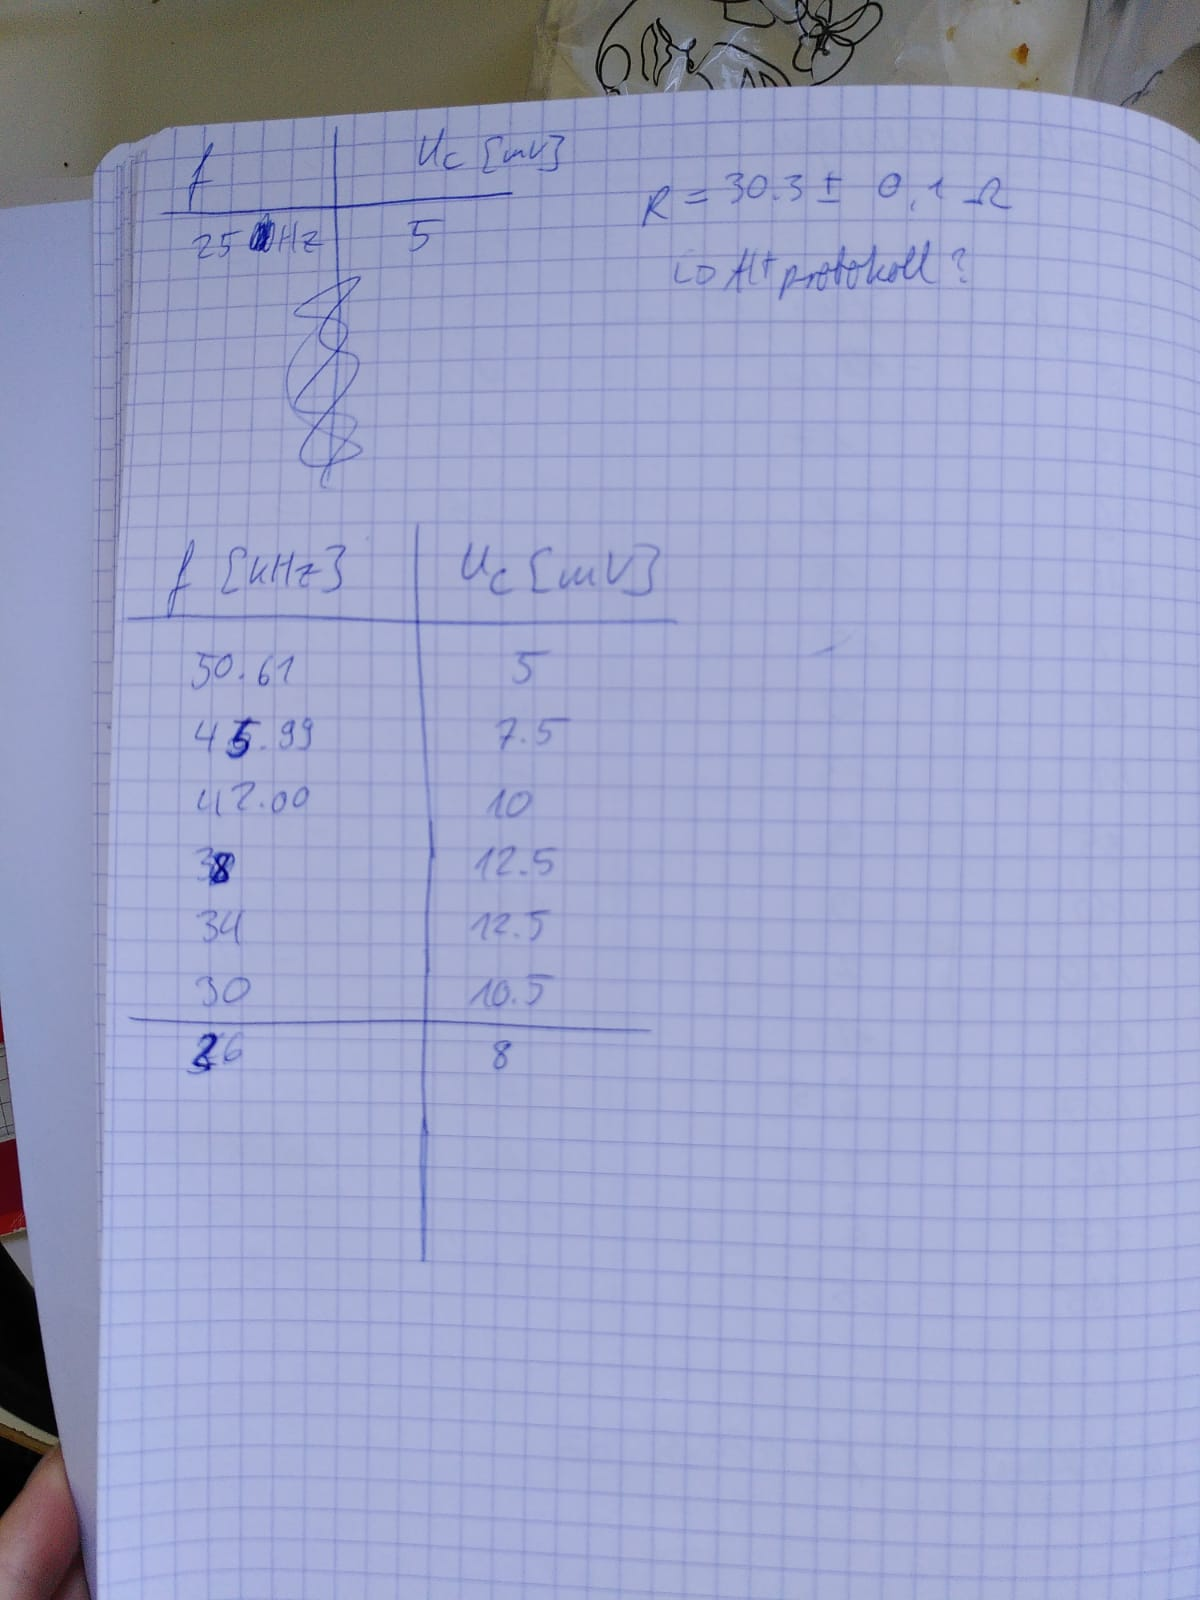
\includegraphics{anhang1.jpeg}
\end{figure}
\begin{figure}
  \centering
  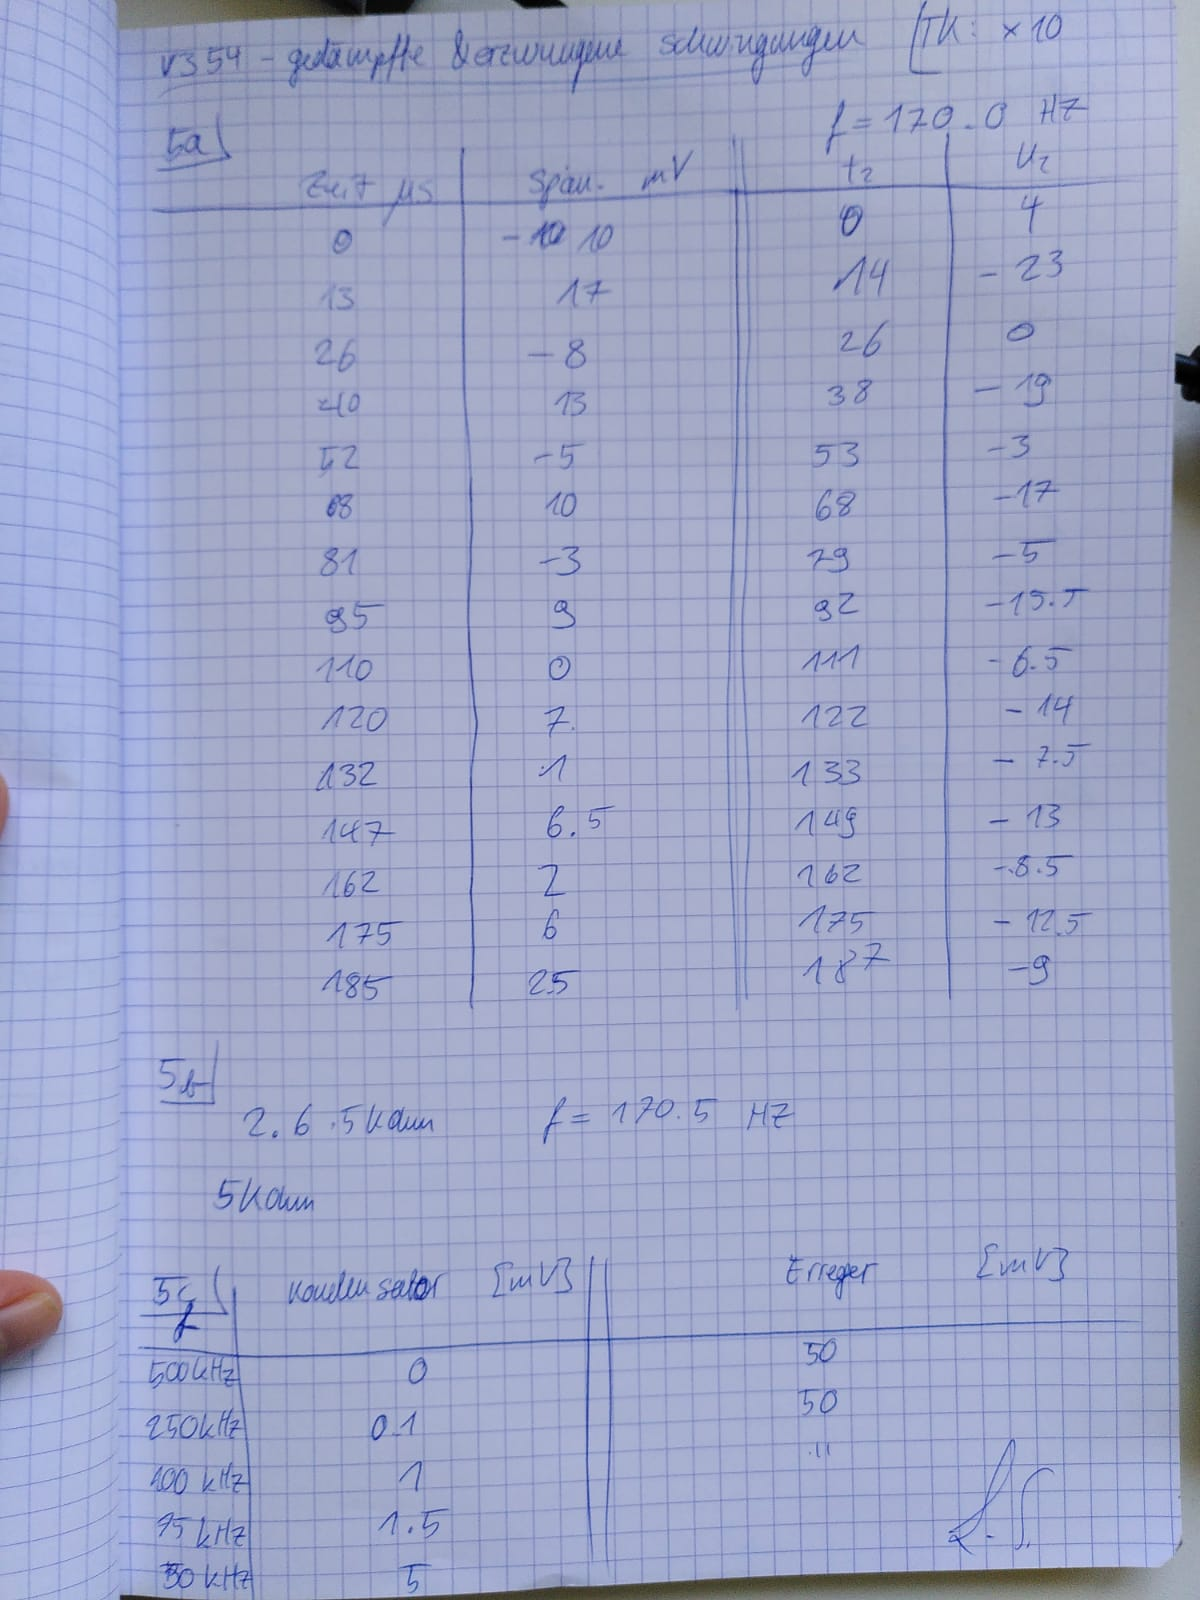
\includegraphics{anhang2.jpeg}
  \caption{Resonanzkurve}
  \label{fig:plot2}
\end{figure}

\end{document}
